\chapter{Solving an exact cover problem instance using the QAOA} \label{ch:qaoa}
\glsreset{qaoa}
In this chapter, we first introduce combinatorial optimization. Next, we explain the \gls{qaoa}, a quantum heuristic algorithm providing approximate solutions to combinatorial optimization problems. We show that using \glspl{carb} can reduce the length of a \gls{qaoa}'s gate sequence implemented on the quantum computer. Next, we demonstrate this advantage experimentally by solving an exact cover problem instance on a three-qubit quantum processor.

\section{Combinatorial optimization}
An optimization problem for which the aim is to find the optimal (or close to optimal) solution amongst a finite set of possibilities is called a \textit{combinatorial optimization problem}.  Such problems are pervasive and appear in applications such as logistics, hardware verification, telecommunication network design, task scheduling and many more~\cite{Sbihi2007CombinatorialA, Coles2018QuantumBeginners, 2014ApplicationsOptimization}.

In its general form, a combinatorial optimization problem is specified by a set of rules, called clauses, acting on strings of $N$ bits, in which each bit represents a binary decision variable~\cite{Farhi2014AAlgorithm}.  Each clause is satisfied for certain assignments of the bits and unsatisfied for other assignments. Solving the problem consists in finding a combination of bits (forming together the bit string, $b := b_1 \, ...\, b_N$) satisfying the largest (weighted) amount of clauses. The objective function can be written as 
\begin{equation} \label{eq:qaoa_clauses}
    C(b) = \sum_{m=1}^M w_m C_m(b)
\end{equation}
where $C_m(b)$ is the $m$-th clause and $w_m$ is its corresponding (real and non-negative) weight. If $C_m(b)$ is satisfied by the bit string $b$ then its value is 1 and otherwise 0. In these terms, solving the problem is expressed as finding the bit string $b_\text{opt}$ maximizing $C$. An approximate solution provides a bit string $b_{\text{approx}}$ for which  $C(b_{\text{approx}})$ is close to the maximum of $C$.

We illustrate this abstract concept with a simple example. Imagine you  have to choose an outfit -- consisting of one t-shirt and one pair of pants -- from your closet. You have 2 shirts to choose from, a white and blue one. Similarly, you have a white and a blue pair of pants. You believe you look better when your whole outfit is of the same color. Additionally, you think your blue shirt suits you better than the white one. Which outfit should you choose for the party? 

While the answer is trivial in this example, we formalize the problem with the terminology introduced above. The outfit, $b = b_1b_2 $, can be formulated as a 2-bit string, one bit for the shirt ($b_1$), and one for the pair of pants ($b_2$). Colors are encoded by the values of the bits: 0 for white and 1 for blue. The four possible outfits are: 00 (white-white), 01 (white-blue), 10 (blue-white) and 11 (blue-blue). The problem has two clauses. $C_1(b) = \neg (b_1 \oplus b_2)$, leading to a value of 1 if you choose a shirt and pair of pants of the same color and 0 otherwise\footnote{$\oplus$ denotes the "XOR" operation and $\neg$ is the logical not.}. $C_2(b) = b_1$ has a value of 1 only if you decide on wearing your blue shirt. The objective function is then:
\begin{equation}
    C(b) = C_1(b) + C_2(b) = \neg (b_1 \oplus b_2) + b_1
\end{equation}
where we assigned equal weights $w_1 = w_2 = 1$ to both clauses.
The score of each output is then:
\begin{subequations}
\begin{equation}
     C(00) = 1 + 0 = 1
\end{equation}
\begin{equation}
    C(01) = 0 + 0 = 0
\end{equation}
  \begin{equation}
      C(10) = 0 +  1 = 1
  \end{equation}
  \begin{equation}
         C(11) = 1 + 1 = 2
  \end{equation}
\end{subequations}

The bit string maximizing $C(b)$ is indeed 11 (blue shirt, blue pants). An algorithm capable of providing this bit string is a combinatorial optimization algorithm. In this case, we used the exhaustive search algorithm, meaning that we enumerated all possible answers and picked the best one. 

In many real applications, exhaustive search is not tractable. In fact, even a slight modification of the presented problem makes it unrealistic to use exhaustive search. Instead of 2, imagine having to choose 25 items, each available in 8 different colors (each item has now 3 bits to encode the colors). The number of possible outfits becomes $2^{3 \cdot 25} \approx 4\cdot 10^{22}$. It would take about a million years to search sequentially through all possibilities for a computer requiring $1\unit{ns}$ to evaluate the cost of each outfit\footnote{Note that you are confronted to a similar situation every morning when dressing up. But you do not use the exhaustive search algorithm to decide what you wear, otherwise you would never get out of your house.}.

Several (classical) heuristic algorithms exist providing an approximate solution for this type of problems. In the next section, we explain the \gls{qaoa}, a quantum heuristic algorithm capable of finding approximate solutions to this type of problems.

\section{The quantum approximate optimization algorithm}\label{sec:qaoa}
The \gls{qaoa}~\cite{Farhi2014AAlgorithm} (depicted in Fig.~\ref{fig:qaoa_scheme}(a)) is a \gls{vqa} designed to find approximate solutions to combinatorial optimization problems. It is a hybrid algorithm executed partially on a quantum computer and partially on a classical computer. 

First, the quantum computer prepares a quantum state $\ket{\vec{\gamma}, \vec{\beta}}$ based on the objective function\footnote{Also often named cost function in the context of a minimization problem.} $C$ characterizing the clauses of the problem (see Eq.~\eqref{eq:qaoa_clauses}), and a set of variational parameters $\theta = (\vec \gamma, \vec \beta)$. The state is prepared with $p$ layers of two unitaries corresponding to the time-evolution of two non-commuting Hamitltonians, $\hat C$ and $\hat B$, applied to a uniform superposition state of $N$ qubits,
\begin{equation}
    |\vec{\gamma}, \vec{\beta}\rangle=\underbrace{\sexp{-\i \beta_{p} \hat B} \sexp{-\i \gamma_{p} \hat C}}_{\text {layer } p} \cdots \underbrace{\sexp{-\i \beta_{1} \hat B} \sexp{-\i \gamma_{1} \hat C}}_{\text {layer } 1}|+\rangle^{\otimes N}
\end{equation}
where  $\ket{+}^{\otimes N} = \left(\frac{1}{\sqrt{2}}(\ket{0}+\ket{1})\right)^{\otimes N}$ is the initialization state, and $\vec\gamma = (\gamma_1, ..., \gamma_p)^\text{T}$ and $\vec\beta = (\beta_1, ... , \beta_p)^\text{T}$ are the real variational parameters for the $p$ layers. Referring to the number of layers, we say that the implementation is of depth $p$. $\hat C$ is the cost Hamiltonian, which for all objective functions of NP-complete problems can be mapped to an Ising Hamiltonian in polynomial time~\cite{Lucas2014IsingProblems},
\begin{equation} \label{eq:ising}
    \hat C =\sum_{n < m} J_{n m} \sigma_{n}^z \sigma_{m}^z + \sum_{n} h_n \sigma_{n}^z
\end{equation}
and $\hat B$ is the mixing Hamiltonian 
\begin{equation}
    \hat B = \sum_{n} \sigma_n^x
\end{equation}
where $\sigma_n^{z}$ ($\sigma_n^{x}$) are the Pauli Z (X) operators applied to the $n$-th qubit, and $h_n$ and $J_{n m}$ are real coefficients. In the combinatorial optimization picture, these coefficients represent the relative weights of each clause, see Eq.~\eqref{eq:qaoa_clauses}.

\begin{figure}[H]
    \centering
    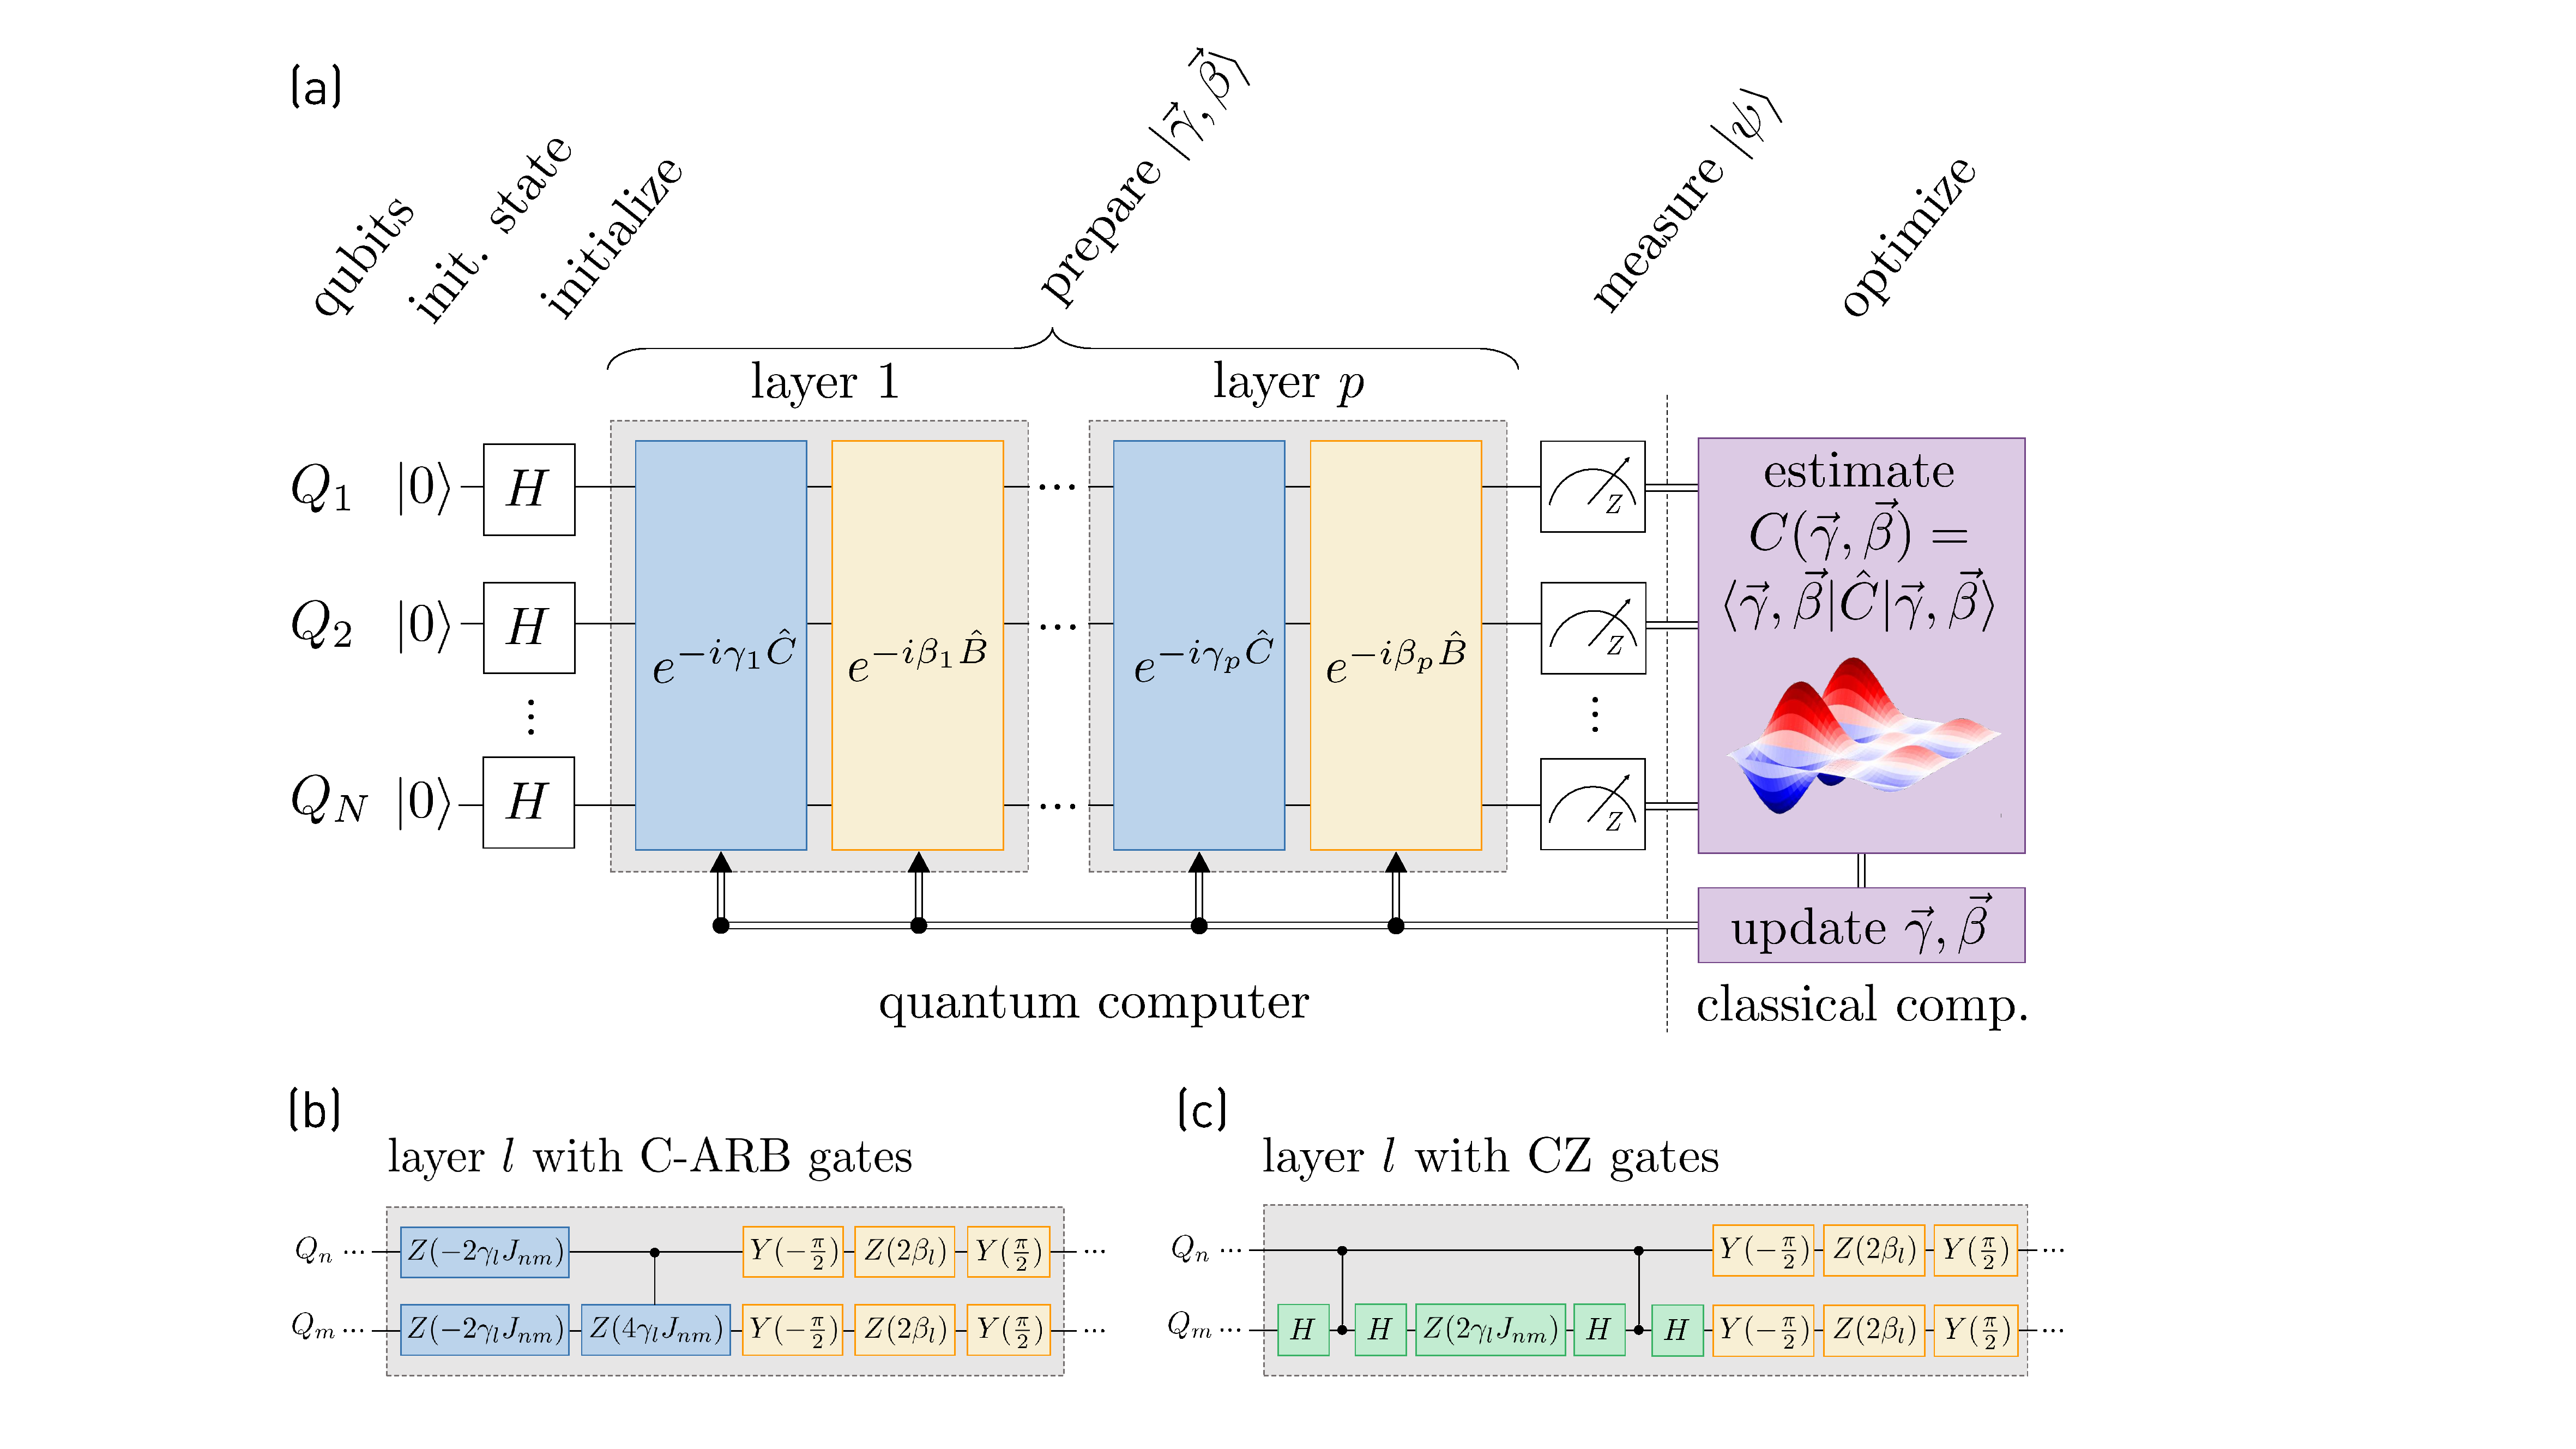
\includegraphics[width=\textwidth, trim ={9cm, 0 15cm, 0}]{chapters/qaoa/figs/qaoa_scheme-v6.pdf}
    \caption{The \gls{qaoa} scheme. $Z(\cdot)$ and $Y(\cdot)$ correspond to single-qubit z- and y-rotations while $H$ is the Hadamard gate. (a) The scheme consists of two steps. First, the quantum computer applies $p$ alternating sequences -- called layers -- of two unitaries corresponding to the time evolution of two Hamiltonians $\hat C$ (blue), $\hat B$ (yellow) scaled by layer-dependent variational parameters to an equal superposition state. The resulting state, \qaoaMeasuredState, is prepared and measured several times to obtain an estimate for the expectation value of a cost function \cost{}, based on the expectation values of single and two-qubit terms. Based on this estimate, a classical optimizer alters the variational parameters to minimize \cost{}. The output of the algorithm is the projection in the z-basis of state \optimalstate{} yielding a bit-string with a low cost. (b) Implementation of a layer of the \gls{qaoa} for a cost Hamiltonian consisting only of two-qubit interaction terms. Only two generic qubits, $Q_n$ and $Q_m$, are represented. The gate's background color indicates which part in (a) it implements. The single-qubit Z gates are virtual gates implemented by adding phase on the subsequent pulses. The two-qubit interaction is mediated by a \gls{carb}. The arbitrary single-qubit x-rotations are not calibrated on the device and are thus decomposed into two y-rotations and a z-rotation. (c) Equivalent gate sequence diagram as in (b) but featuring a decomposition of the \gls{carb} into \glspl{cz} and single-qubit gates.}
    \label{fig:qaoa_scheme}
\end{figure}

The resulting state \qaoaMeasuredState{} is measured in the $Z$ basis. A classical computer uses the measurement outcome (i.e.\ bit strings corresponding to the eigenstates of \qaoaMeasuredState{}) to compute the expectation value of $\hat C$ and iteratively updates the variational angles to optimize the objective function. When the objective function is mapped to the Ising Hamiltonian, the resulting problem consists in finding the lowest energy state of the system, i.e.\ minimizing the expectation value of the cost Hamiltonian. Once the optimizer has converged, the state \optimalstate{} constitutes an approximate solution for the optimization problem.

\subsection{Success probability} \label{sec:qaoa_success_prob}
Measuring successive preparations of \optimalstate{} yields a distribution on the eigenstates $\ket{\psi_i}$.
We define the success probability, $P_s$, as the probability of measuring an eigenstate that is a solution to the combinatorial problem. 

Note that the optimization is performed on the smooth landscape of the objective function \cost{} and not on $P_s$ directly. But for problems with a discrete domain of real values, a low expectation value of the cost function generally guarantees a high concentration of probability on optimal solutions upon measurement~\cite{Cook2019TheCover, Wang2019XY-mixers:QAOA}.

\subsection{Layer implementation}
The algorithm is subdivided into layers, in which each layer $l$ includes the unitary $\sexp{-\i\gamma_l\hat C}$. Since $\hat C$ is diagonal in the computational basis, all its terms commute. In addition, in this thesis we consider the case where all $h_n = 0$. Therefore, we look at the implementation of a single generic term $J_{nm}\sigma_n^z\sigma_m^z$ involving qubit $Q_n$ and qubit $Q_m$. Any other term in $\hat C$ can be applied before or after in the exact same way. 

The corresponding unitary to implement is $\sexp{-\i J_{nm} \gamma_l \sigma_n^z\sigma_m^z}$, yielding in the $nm$-two-qubit subspace,
\begin{equation} \label{eq:qaoa_two_qubit_cost_unitary}
    U_{nm}^l = 
    \begin{pmatrix}
    \sexp{-\i\gamma_l J_{nm}} & 0 & 0 & 0\\
    0 & \sexp{\i\gamma_l J_{nm}} & 0 & 0 \\
    0 & 0 & \sexp{\i\gamma_l J_{nm}} & 0 \\
    0 & 0 & 0 & \sexp{-\i\gamma_l J_{nm}}
    \end{pmatrix}
\end{equation}{}
We present two approaches to implement this unitary. The first one, which we call the \textit{\gls{dir}}, implements Eq.~\eqref{eq:qaoa_two_qubit_cost_unitary} with a single \gls{carb} and two single-qubit $Z$-gates (see Fig.~\ref{fig:qaoa_scheme}(b)). The \gls{carb} introduces a phase of $4\gamma_l J_{nm}$ on the \oo{} state which is then redistributed to the other diagonal terms by single-qubit $Z$-gates rotating their respective qubit subspace in the opposite direction with half the angle, i.e.\ $2\gamma_l J_{nm}$. Up to a global phase, this implements Eq.~\eqref{eq:qaoa_two_qubit_cost_unitary}. Note that, due to the presence of the variational parameter $\gamma_l$, the angle on the \oo{} state may have any real value and therefore indeed requires a \gls{carb} to rotate the \oo{} state with a single gate.

In case we choose to limit the gate set to the use of \glspl{cz} only (i.e.\ rotation of $\pi$ on the \oo{} state), we use a \textit{\gls{dec} } consisting of two \glspl{cz} and additional single-qubit gates (see green colored elements in Fig.~\ref{fig:qaoa_scheme}(c)).

In Section~\ref{sec:qaoa_experiment}, we compare experimentally the performance of both implementations.

\subsection{Relation to adiabatic quantum computing}\label{sec:qaoa_relation_to_adiabiatic_computing}
The depth $p$ of a \gls{qaoa} implementation is defined as the number of layers used for the state preparation. This parameter plays an important role both in theory and in experiments.

For $p \rightarrow \infty$, the \gls{qaoa} finds the global optimium of $C$~\cite{Farhi2014AAlgorithm}. Intuitively, this is because the \gls{qaoa} can be seen as a Trotterized approximation~\cite{TrotterMathematics} of the quantum adiabatic algorithm~\cite{Farhi2000QuantumEvolution}. Similarly to the \gls{qaoa}, the quantum adiabatic algorithm starts in the lowest energy state of the mixing Hamiltonian $\hat B$, i.e.\ the equal superposition over all qubits in the $Z$ basis, and then evolves adiabatically to the lowest eigenstate of the cost Hamiltonian $\hat C$. The time-dependent Hamiltonian during this evolution is

\begin{equation} \label{eq:qaoa_adiabatic_evolution}
 \hat H(t)=\hat H_1(t) +\, \hat H_2(t) = (1-t / T) \hat B + \, (t / T) \hat C
 \end{equation}
where $T$ is a real and positive parameter called run time. As long as the evolution is sufficiently slow i.e.\ $T$ is sufficiently large, this process forces the state of the system to remain in the ground state of the slowly varying Hamiltonian $\hat H(t)$, ultimately resulting to the ground state of $\hat C$~\cite{Farhi2000QuantumEvolution, Farhi2014AAlgorithm}. 

To implement this on a quantum computer, we break down the total time evolution $U(0, T)$ from 0 to $T$ into $K$ smaller intervals $U_k((k-1)\Delta t,\, k\Delta t)$ of length $\Delta t$ such that
\begin{equation} \label{eq:qaoa_discretized_adiabatic_evolution}
    \ket{\psi_{\textrm{opt}}} = U(0, T)\ket{+}^{\otimes N} = U_K((K-1)\Delta t, \,K\Delta t) ... U_0(0,\, \Delta t) \ket{+}^{\otimes N}
\end{equation}
with the time evolution in each interval given by 
\begin{equation}
    U_k(k\Delta t, (k+1)\Delta t) = \mathcal{T}\exp{\left(-\i\int_{k\Delta t}^{(k+1)\Delta t} \hat H(t)\d t\right)}
\end{equation}
 and the time ordering operator $\mathcal{T}$~\cite[p. 143]{Weinberg1995TheFields}. It is shown that removing the time ordering operator introduces an error $\epsilon \propto \Delta t^2$~\cite{Poulin2011QuantumSpace}. Intuitively, this suggests that as long as the time intervals are small, the order of operations within the step leads to negligible errors. It is also more practical to approximate the integral by a sum, for instance using Monte-Carlo integration~\cite{Poulin2011QuantumSpace}. The latter replaces the integral by the average of $M$ evaluations of the function at random times $\tau_m^k$ within the interval $\Delta t$ which introduces an error $\epsilon_{\textrm{MC}} \propto \Delta t/\sqrt{M}$. The time evolution step becomes
 \begin{equation}
     U_k(k\Delta t, (k+1)\Delta t) = \exp{\left(-\frac{\i}{M}\sum_{m=1 }^{M} \hat H(\tau_m))\right)} =  \prod_{m=1}^M \sexp{-\frac{\i}{M}\hat H(\tau_m^k)}
 \end{equation}
 Within the product, the Hamiltonian is not time dependent anymore, such that we can apply the Trotter formula to decompose it into the two components $\hat B$ and $\hat C$. 
 The Trotter product formula stipulates for two non-commuting time-independent Hamiltonians $\hat H_1$ and $\hat H_2$~\cite{TrotterMathematics}:
\begin{equation} \label{eq:qaoa_product_formula}
    \sexp{-\i\left(\hat H_{1} + \hat H_{2}\right) t}=\lim _{N \rightarrow \infty}\left(\sexp{-\i \hat H_{1} t / N} \sexp{-\i \hat H_{2} t / N}\right)^{N}
\end{equation}
Truncating this equation to a finite value for $N$ yields an error with lowest order term in $\mathcal{O}\left(\frac{t^2}{2N} [\hat H_1, \hat H_2]\right)$~\cite{Heyl2018QuantumSimulation, Lloyd1996UniversalSimulators}. 

In this case, we make an approximation of order $N=1$ with $\hat H_1 = (1-\frac{\tau_m^k}{T})\hat B$ and $\hat H_2 = \frac{\tau_m}{T} \hat C$. The full adiabatic evolution of Eq.~\eqref{eq:qaoa_discretized_adiabatic_evolution} becomes the alternating sequence between the two Hamiltonians $\hat B$ and $\hat C$,
\begin{equation} \label{eq:qaoa_prod_formula}
    U(0,T) = \prod_{k=0}^{K-1} U_k(k\Delta t, \,(k+1)\Delta t)= \prod_{k=0}^{K-1}\prod_{m=1}^M \sexp{-\i\frac{ \overbrace{1-\tau_m^k/T}^{\beta_{km}}}{M}\hat B}\sexp{-\i\frac{\overbrace{\tau_m^k/T}^{\gamma_{km}}}{M}\hat C}
\end{equation}
Note that applying this discretized adiabatic time evolution on $\ket{+}^{\otimes N}$ as presented in Eq.~\eqref{eq:qaoa_discretized_adiabatic_evolution} ends in the global extremum of $\hat C$ \textit{only} for $K \rightarrow \infty$ and large $T$. In that case, the number of layers is given by $p = K\cdot M$ and corresponds intuitively to approximating the time evolution from 0 to $T$ by infinitely many time steps. The error in the approximation of the integral intrinsically tends to zero if $\Delta t \rightarrow 0$. In such a scenario, the  set of variational parameters $(\vec\gamma, \vec\beta) = \{(\gamma_0, \beta_0), ... (\gamma_p, \beta_p)\}$ highlighted in Eq.~\eqref{eq:qaoa_prod_formula} suffices to find the optimum. 

However, in practice the number of layers we can implement on a quantum computer is limited. Therefore, we truncate Eq.~\eqref{eq:qaoa_prod_formula} to a finite value for both $K$ and $M$. This truncation introduces approximation errors and finding the global optimum is no longer guaranteed. 

To mitigate this approximation, we relax the adiabatic constraint ($\beta_l = 1 - \gamma_l$) at each layer to allow for a potentially more direct path to the ground state than the adiabatic one. By optimizing these parameters at each layer variationally, the \gls{qaoa} can reach the ground state with high accuracy for some problem instances even with a relatively small number of layers~\cite{Moll2017QuantumDevices}. 

\subsection{Quantum speedup and the importance of depth}
At the time of its first publication, the \gls{qaoa} achieved a higher approximation ratio on MAX-3-LIN-2 -- a specific instance of the NP-complete MaxCut problem~\cite{GareyM1990} -- than any other classical algorithm. This is no longer the case~\cite{Barak2015BeatingDegree, Hastings2019CLASSICALALGORITHMS}. In fact, several research articles have shown that classical algorithms could outperform the \gls{qaoa} on a variety of problem instances~\cite{Barak2015BeatingDegree, Hastings2019CLASSICALALGORITHMS, Bravyi2019ObstaclesProtection}. On the other hand, several articles claim to achieve Grover speedup for unstructured search~\cite{Jiang2017Near-optimalField} and state transfer~\cite{Niu2019OptimizingDepth} using the \gls{qaoa}. Whether or not the \gls{qaoa} will provide a provable or practical speedup compared to classical algorithms remains unanswered. 

Understanding the number of layers required to open a path to the ground state as function of (i) the number of qubits in the Hamiltonian, and (ii) the chosen problem instance are both open research questions. In addition, it remains unclear whether the path can be found efficiently as the number of variational parameters grows with $2p$. Early results suggests that, for \gls{qaoa} to provide any quantum speedup, the scaling of $p$ must be faster than $\mathcal{O}(1)$ otherwise the circuit is likely simulated efficiently on a classical computer~\cite{Bravyi2019ObstaclesProtection}. On the other hand, to ensure a quantum speedup the scaling of $p$ should also not grow faster than $\mathcal{O}(\log N))$ because faster scaling could imply that finding good variational parameters becomes exponentially hard~\cite{Cerezo2020Cost-Function-DependentNetworks}. 

While the above considerations provide insights into the theoretical performance of the \gls{qaoa} as function of depth, they do not provide insights into the experimental performance on \gls{nisq} devices. In this work, we highlight a crucial experimental trade-off related to the number of layers. Namely, in theory the performance of \gls{qaoa} circuits can only improve with increasing number of layers~\cite{ZhouQuantumDevices}. However, the performance on near-term quantum computers will not increase monotonically with depth due to decoherence and other noise sources. There will be an optimal number of layers beyond which additional layers only decrease the performance of the algorithm. We illustrate this trade-off in the next section and show that the \gls{dir} increases the number of layers which can be executed reliably compared to the \gls{dec}
This in turn allows to solve more complex problem instances using the \gls{dir}

\section{Exact cover} \label{sec:qaoa_exact_cover}
We choose to solve an instance of the exact cover problem~\cite{Karp1972ReducibilityProblems} to compare the direct and decomposed implementation of \gls{qaoa}. The exact cover is NP-complete~\cite{GareyM1990}, meaning that there is no known algorithm to find answers in polynomial time\footnote{An algorithm runs in polynomial time if its execution time, in the worst case scenario, is upper-bounded by a polynomial function of the input $N$, i.e.\ its time complexity scales as $\mathcal{O}(N^k)$ with $k$ a positive and real constant.}, but answers can be checked in polynomial time. In other words, the problem is "hard to solve" but it is "easy" to check the validity of a proposed solution. In addition, the NP-completeness guarantees that any problem in NP can be reduced to the exact cover in polynomial time, such that studying the exact cover is closely related to studying other NP problems. Finally, the exact cover can be easily construct via a problem graph that is not complete, which allows to create instances respecting the hardware connectivity of the quantum device (see Chapter~\ref{ch:outlook} for a discussion on hardware connectivity).

In this section, we provide the formal definition of the exact cover and introduce a problem instance which we the solve in Section~\ref{sec:qaoa_experiment} using \gls{qaoa}. 

\subsection{Definition}
The exact cover is an NP-complete decision problem formulated as follows: \textit{given a set $\mathcal{N}$, and a collection $\mathcal{L}$ of subsets of $\mathcal{N}$, is there a subcollection $\mathcal{L}'$ of $\mathcal{L}$ for which each element in $\mathcal{N}$ is included exactly once?} In other words, elements of the subcollection $\mathcal{L}'$ must be disjoint and their union must be $\mathcal{N}$.

As mentioned in Section~\ref{sec:qaoa}, any NP-complete problem can be mapped onto an Ising Hamiltonian in polynomial time. For the exact cover, this is most conveniently done using an incidence matrix $M$~\cite{WeissteinIncidenceMatrix}, where each row corresponds to an element of $\mathcal{L}$ and each column to an element of $\mathcal{N}$. The matrix element $M_{ln}$ is equal to 1 if the $l$-th element of $\mathcal{L}$ contains the $n$-th element of $\mathcal{N}$ and 0 otherwise.
The Ising parameters $J_{nl}$ and $h_l$ are obtained from $M$~\cite{Lucas2014IsingProblems, Vikstal2019ApplyingProblem}:
\begin{subequations}
\begin{equation}
    J_{l n}=\frac{1}{2} \sum_{k=1}^{N} M_{l k} M_{n k}
\end{equation}
\begin{equation}
h_{l}=\frac{1}{2} \sum_{n=1}^{N} M_{l n}\left(\sum_{k=1}^{L} M_{k n}-2\right)
\end{equation}
\end{subequations}
This formulation requires $L = |\mathcal{L}|$ binary variables $\{b_1, ..., b_L\}$ with $b_l\in\{0,1\}$. To yield an Ising Hamiltonian formulation, see Eq.~\eqref{eq:ising}, each binary variable $b_l$ is mapped to a spin variable $\sigma_l \in \{-1,1\}$ with the mapping, 
\begin{equation}
\sigma_l = 1 - 2 b_l
\end{equation}
Finally, each spin in the problem is modelled by a qubit on the quantum processor. 

\subsection{Example problem instance}
In this work, we consider the 3-qubit problem instance depicted in Fig.~\ref{fig:qaoa_exact_cover_matrix}.  $\mathcal{N} := \{1,2,3\}$ and the elements of $\mathcal{L}$ are $A := \{1,2\},\,\, B := \{1,2,3\}$ and $C := \{2,3\}$, encoded in qubit 1, 2 and 3 respectively. In this picture, the decision problem becomes: \textit{is there a subcollection $\mathcal{L}'$ of letters for which each number in $\mathcal{N}$ is included exactly once?} The answer is yes, and the corresponding subcollections are $\mathcal{L}_1' = \{A,C\}$ and $\mathcal{L}_2' = \{B\}$. These subcollections are encoded in the states $\ket{\psi}=\ket{101}$ and $\ket{010}$, where a 1 in position $l$ indicates that the $l$-th element of $\mathcal{L}$ is included in the subcollection $\mathcal{L'}$.

"Solving" this problem instance corresponds to measuring $\ket{\psi}=\ket{010}$ and $\ket{\psi}=\ket{101}$ with high probability as measuring and checking whether this state is part of the solution set would allow to answer the yes/no-decision problem.

The cost Hamiltonian of the problem is
\begin{equation}
    \hat C = \frac{1}{2}\hat\sigma_1^z\hat\sigma_2^z + \hat\sigma_2^z\hat\sigma_3^z
\end{equation}
and the corresponding cost function $\cost = \bra{\vec\gamma, \vec\beta} \hat C \qaoaMeasuredState{}$ reaches its minimum value of $\cost = -1.5$ when $\qaoaMeasuredState{} = \ket{101}$ or $\ket{010}$. 

\begin{figure}[t]
    \centering
    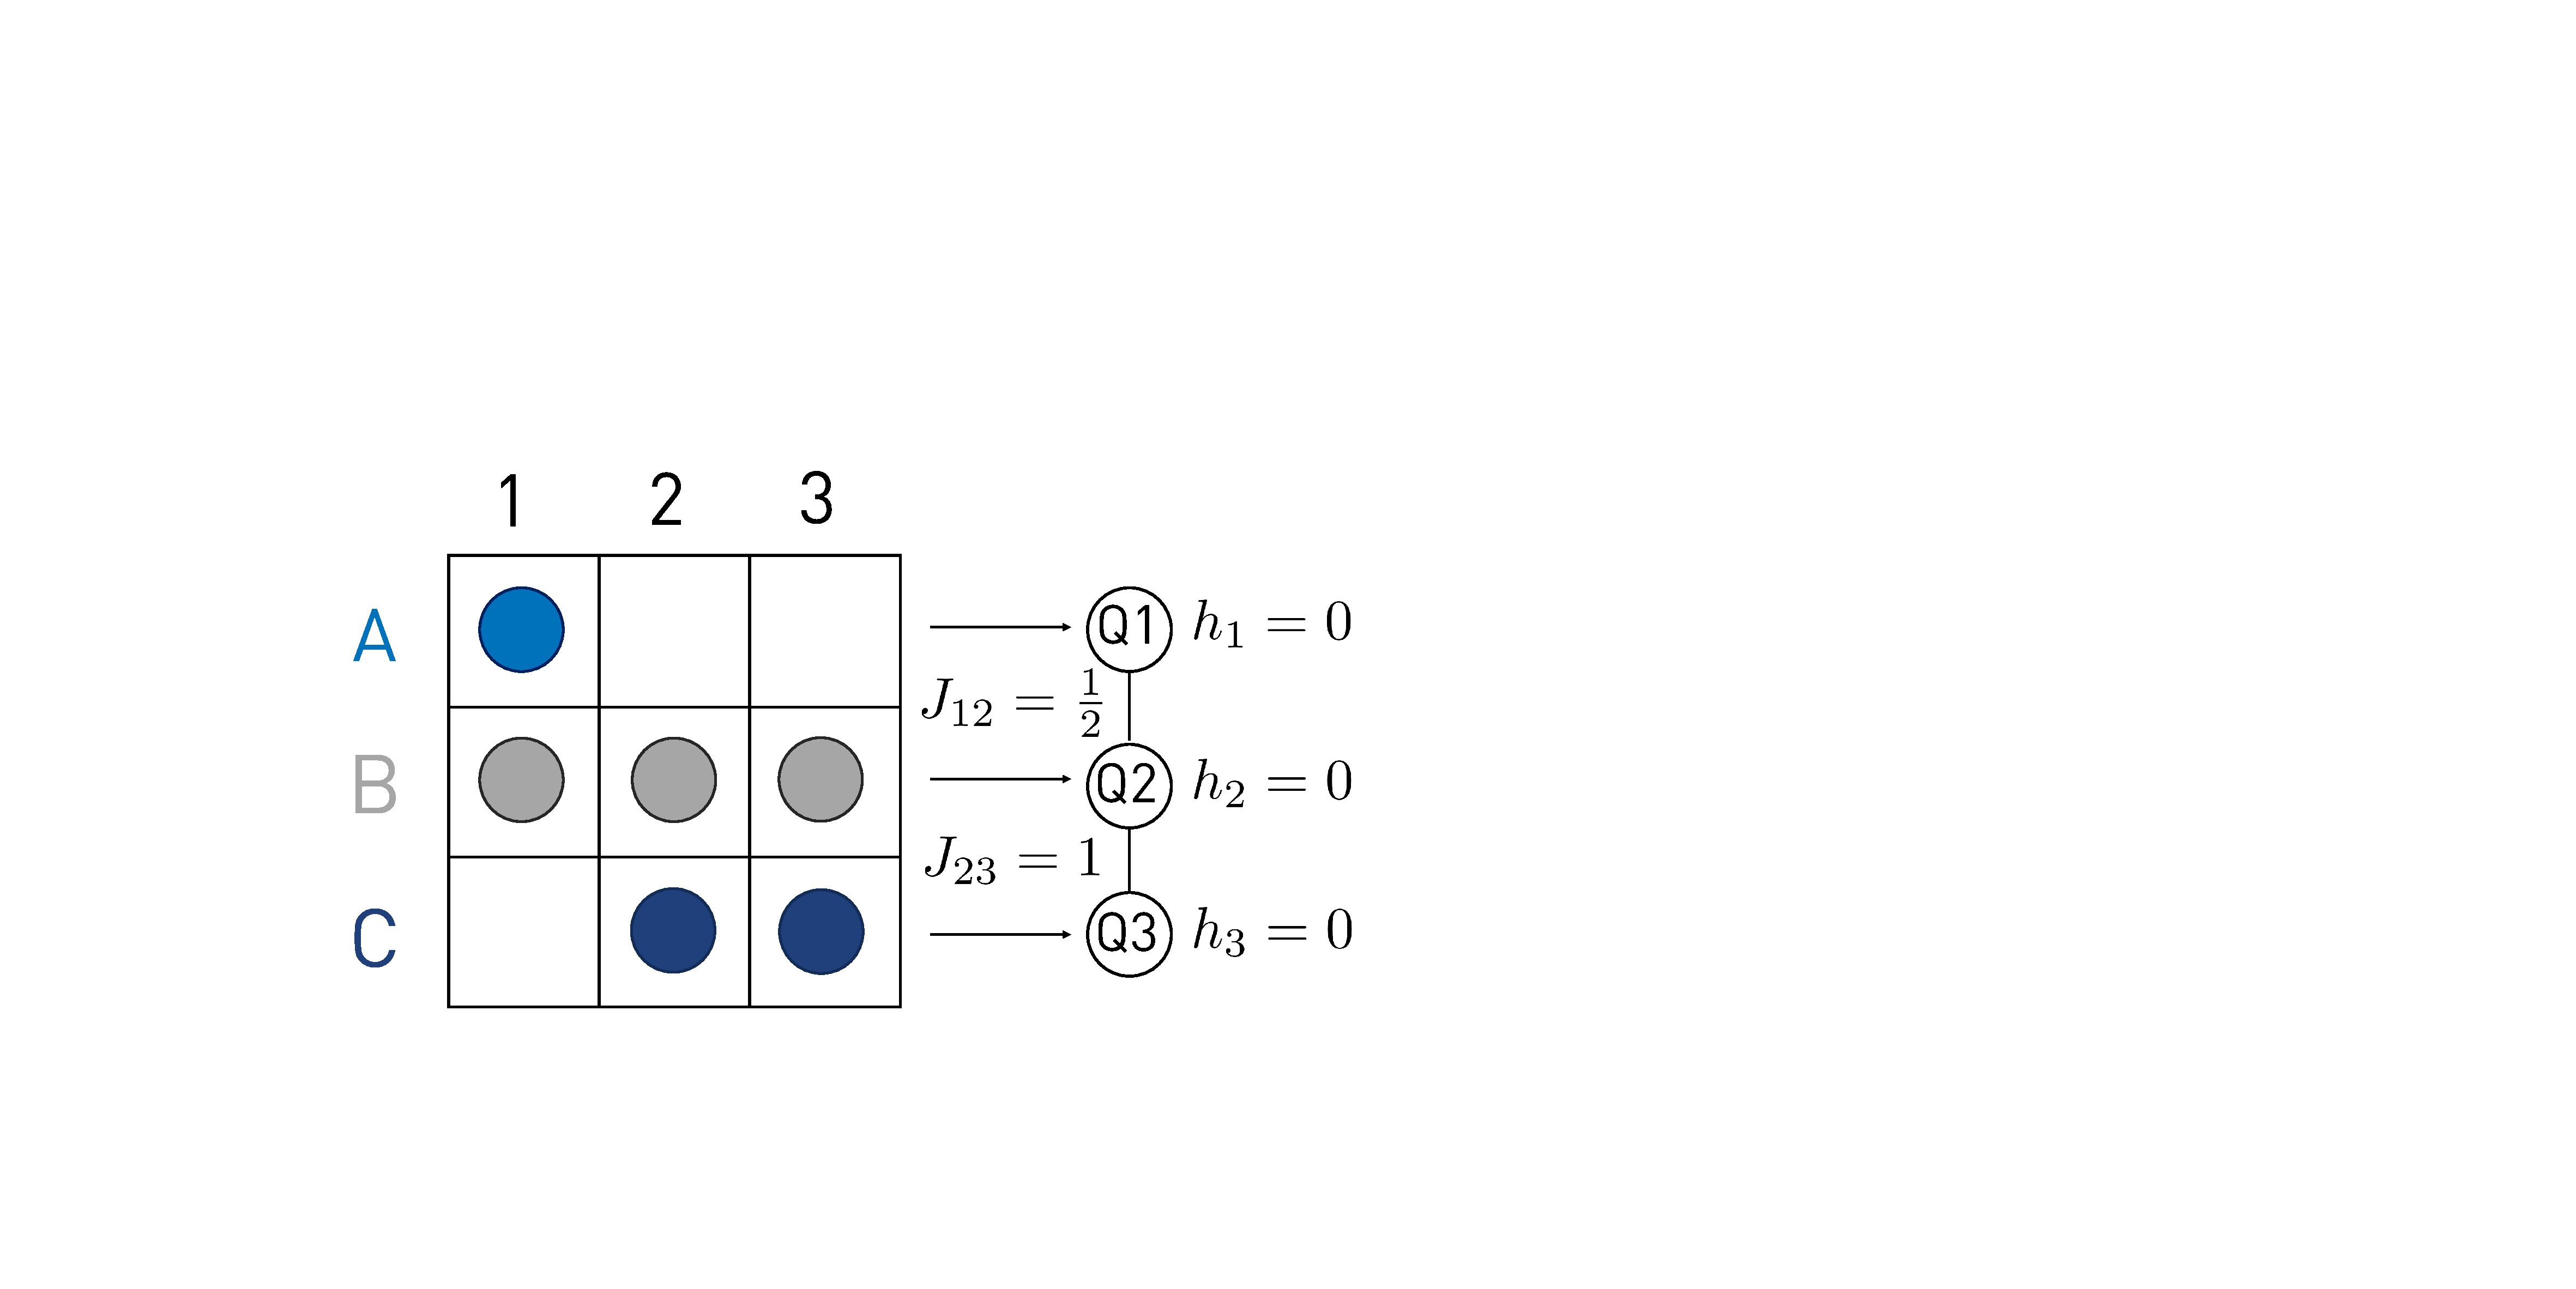
\includegraphics[width=0.8\textwidth, trim={11cm 8cm 38cm 13cm},clip]{chapters/qaoa/figs/exact_cover_matrix.pdf}
    \caption{Incidence matrix representation of the exact cover problem instance implemented in this work. A dot indicates a 1 and an empty square indicates a 0. The mapping to the 3 qubit chain and the corresponding Ising Hamiltonian parameters are indicated on the right hand side.}
    \label{fig:qaoa_exact_cover_matrix}
\end{figure}

\section{Experiment} \label{sec:qaoa_experiment}
In this section, we implement the \gls{qaoa} on a quantum processor to find an approximate solution to a combinatorial optimization problem with 3 qubits. In addition, we compare the performance of the \gls{dir} and \gls{dec} for different depths. We use qubits 1, 2 and 3 of the device presented in Appendix~\ref{app:setup}. Information relative to the single- and two-qubit gates are reported in Appendix~\ref{app:setup}, Table~\ref{tab:cz_gate_params}. All measurements are performed with 3-level single shot readout, see Appendix~\ref{ch:qutrit_readout}. In the context of the \gls{qaoa}, leakage events can be seen as measuring bit strings which do not belong to the space of possible solutions. We therefore condition the measurements outcome on no leakage event. Hence, leakage events reduce the effective number of shots on which we compute estimates. They do not, however, influence the algorithm as long as as the excitation stays in the \f{} level until the state is measured. We make this assumption, as sequences of interest are shorter than $4\,\mu\text{s}$, and the shortest \f{} level $T_1$ is approximately $10\,\mu\text{s}$. All measurements are done without ground state heralding or readout error correction.

\subsection{Cost function landscapes}
Although $p=1$ does not always yield a good approximate solution to the optimization problem, it is a useful intermediate benchmark towards implementing multi-layer \gls{qaoa} circuits ~\cite{Pagano2019QuantumSimulator, Bengtsson2019QuantumProcessor}. A single layer implementation has two variational parameters, $\gamma$ and $\beta$, such that the cost function landscape can be mapped out and visualized with a grid search over $\gamma$ and $\beta$. We make several observations to restrict the search space for each parameter. 

First, if $\hat C$ has only integer eigenvalues\footnote{$\hat C$ is diagonal and therefore elements on its diagonal are the eigenvalues by definition.}, then $\gamma$ is at least $2\pi$-periodic because $\sexp{-\i(\gamma + 2\pi) \hat C} = \sexp{-\i 2\pi \hat C} \sexp{-\i \gamma \hat C} = \sexp{-\i \gamma \hat C}$ since $2\pi \hat C$ yields integer multiples of $2\pi$ for all elements on the diagonal. If in addition the eigenvalues are either all odd or all even, then $\gamma$ shows a periodicity of $\pi$, as $\sexp{i\pi\hat C}$ yields in that case $\pm I$ depending on whether the eigenvalues are all odd or all even. By construction, this is the case when all $J_{nm}$ in $\hat C$ are integers. 

Second, the parameter $\beta$ yields single-qubit $x$-rotations of angle $2\beta$ on all qubits and is therefore at least $\pi$-periodic.

We thus restrict our search space for this problem instance\footnote{In the problem instance we study, the eigenvalues are odd integers multiples of 1/2 and not odd integers. Therefore, the periodicity in $\gamma$ is only $2\pi$ and not $\pi$. We make use of the fact that the landscape is point symmetric around ($\gamma$, $\beta$) = ($\pi$, $\pi/2$) due to the linear connectivity to restrict the search space of $\gamma$ between 0 and $\pi$. Another option would have been to multiply $\hat C$ by a constant factor such that all eigenvalues are integers.} to the domain $(\gamma, \beta) \in [0, \pi] \,\times\, [0, \pi]$. For each parameter pair, we repeat the state preparation and measurement 20000 times to estimate the expectations values $\langle\szsz{1}{2}\rangle$ and $\langle \szsz{2}{3} \rangle$ from which the cost \cost{} is computed.

We execute this measurement with a resolution of 45 points per axis both for the \gls{dir} and the \gls{dec}, and present the result in Fig.~\ref{fig:qaoa_landscapes} along with the landscape obtained with a noise-free unitary evolution (which does not take into account decay and dephasing rates) simulated in QuTip~\cite{Johansson2013QuTiPSystems} .

The simulation reveals two global minima for \cost{} $\approx -1.05$ at $(\gamma, \beta) \approx (\frac{2\pi}{9}, \frac{\pi}{7})$ and $(\frac{2\pi}{9},\pi/2 + \frac{\pi}{7})$.  The landscape also exhibits two pairs of local minima with slightly different depths; one at $\gamma \approx \frac{5\pi}{8}$ and one at $\gamma \approx \frac{7\pi}{8}$ also separated by $\pi/2$ in the $\beta$ direction. The $\pi/2$ periodicity in $\beta$ can be understood intuitively from the Bloch sphere perspective: for $p=1$, we start on the equator and apply parametrized entangling $Z$-rotation between qubits. Each qubit therefore stays on the equator of its Bloch sphere. Thereafter, we apply parametrized $X$-rotations on all qubits which rotate the vectors back towards the $z$-axis\footnote{Except if the vectors are degenerate with the $\pm x$-axis.}. For a $X$-rotation angle larger than $\pi$ (i.e.\ $\beta>\pi/2$), we simply inverse the polarity of all states (all $\ket{1}$ are now mapped to $\ket{0}$ and vice-versa). The correlations between qubits remain unaffected by this polarity inversion and therefore the landscape is periodic.

The locations of all extrema in the measurements are in good agreement with the simulations, suggesting a low amount of total coherent errors. Incoherent errors due to decoherence affect the contrast of the landscapes, resulting in a minimum measured cost of $\sim -0.95$ ($\sim -0.85$) for the direct (decomposed) implementation. The decomposed implementation does not reach the same cost value as its gate sequence is longer and thereby more affected by decoherence. In addition, it suffers more from coherent errors than the direct implementation. The latter are caused predominantly by residual $ZZ$-coupling, and therefore accumulate over the longer sequence. The combination of these effects could explain the diagonal feature observed in its landscape, which does not appear as strongly for the direct implementation. The average total leakage (any qubit measured in the \f-level) amounts to 4.5\% for the direct implementation and 7.8\% for the decomposed implementation. Most of the leakage occurs due to the two-qubit gate between qubit 1 and qubit 2, which suffers from higher leakage (see Appendix~\ref{app:setup}, Table~ \ref{tab:cz_gate_params} for a detailed discussion).

Note that even in the noise-free simulation, \cost{} never reaches its minimum value of -1.5 thereby indicating that the performance of the algorithm is limited by the chosen depth of $p=1$. Nevertheless, additional layers introduce new variational parameters, making grid search quickly intractable. Therefore, we use a classical optimizer to find the optimal variational parameters.

\begin{figure}[ht]
    \centering
    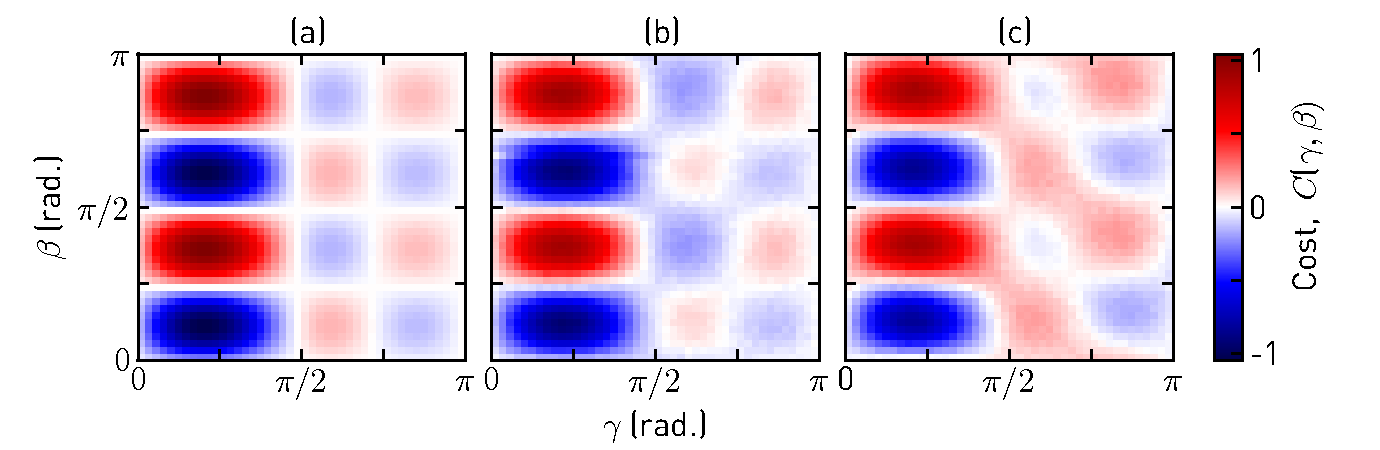
\includegraphics[width=\textwidth]{chapters/qaoa/figs/qaoa_landscapes_20200216_211657.pdf}
    \caption{Optimization landscapes for a \gls{qaoa} implementation with one layer. The two variational parameters, $\gamma$ and $\beta$ are swept over a 45x45 grid, and the cost function $\cost$ is evaluated for each parameter pair.  (a) Landscape obtained with noise-free simulation. The minimal cost function value is approximately -1.05. (b) Landscape obtained with the direct implementation of the \gls{carb}. Taken with 20000 single shot measurements per parameter pair. (c) Landscape obtained with the decomposed implementation of the \gls{carb}. Taken with 20000 single shot measurements per parameter pair. }
    \label{fig:qaoa_landscapes}
\end{figure}


\subsection{Variational parameter optimization} \label{sec:qaoa_optimization}
When no strategy is known to find the best variational angles and  $p > 1$,  classical optimizers constitute a way to navigate through the parameter space. Desirable properties to ensure rapid and consistent convergence to the optimal parameters are:
\begin{itemize}
    \item [--] \textbf{Low cost function sampling}. Each query to the quantum computer is costly in time. Therefore, optimizers minimizing the number of queries sent to the quantum computer are better suited for this task. Algorithms relying on Hessian matrix estimation are not suited, as the number of elements in the Hessian matrix grows quadratically with $p$.
    \item[--] \textbf{Robustness to noise}. Measurements from quantum computers are subject to noise. Especially when the gradient of the cost function is small, it is crucial for the algorithm to be robust to fluctuations.
    \item[--] \textbf{Capability of avoiding local minima}. At low depths, the cost functions show local minima. Algorithms capable of finding the global optimum are better suited.
\end{itemize}

We leave the task of finding the optimal classical optimizer for future work, and instead focus on comparing the performance difference of a simple optimizer between the \gls{dir} and \gls{dec}
For the sake of completeness, we briefly report on optimizers which have been applied to \gls{qaoa} in recent literature.

To find variational parameters for a single layer \gls{qaoa} implementation, Ref.~\cite{Otterbach2017UnsupervisedComputer} applied Bayesian optimization (BO)~\cite{Mockus1989GlobalApproach}, a gradient-free, global optimization method relying on Gaussian processes. Although BO performs excellently in low-dimensional parameter spaces, the number of evaluations grows exponentially with the number of parameters, rendering it impractical when $p$ is large. Ref.~\cite{Bengtsson2019QuantumProcessor} compared BO on a two-layer \gls{qaoa} implementation with the Nelder-Mead (NM) algorithm~\cite{Nelder1965AMinimization} and the covariance matrix adaptation evolution strategy (CMA-ES)~\cite{Hansen2016TheTutorial}. On their problem instance, NM has the lowest cost function sampling but is also the most sensitive to local minima due to its locality. By contrast, the CMA-ES requires more function evaluations but is stochastic and is believed to scale favorably with the number of parameters~\cite{Bengtsson2019QuantumProcessor}. For $p=2$, BO yielded a good trade-off between low cost function sampling and sensitivity to local minima. 
Ref.~\cite{Pagano2019QuantumSimulator} used problem-specific heuristics combined with a bootstrapping algorithm. Other heuristics~\cite{ZhouQuantumDevices} and deep-learning based approaches~\cite{Verdon2019LearningNetworks} have been proposed but not tested beyond simulations. Finally, the simultaneous perturbation stochastic approximation (SPSA)~\cite{Bhatnagar2013StochasticOptimization} is a promising stochastic global optimization approach not yet applied to \gls{qaoa}. The major advantage of SPSA is that it requires only two cost function evaluations per optimization step, independently of the dimensions of the parameter space.

In this work, we use the NM algorithm, due to its simplicity and low cost function sampling. To mitigate the effect of local minima, we increase the size of the initial simplex to the same order of magnitude as the distance between minima observed in Fig.~\ref{fig:qaoa_landscapes}.

 For each optimization trajectory, we initialize parameters randomly and then let the NM algorithm run 40 cost function evaluations. One function evaluation takes approximately 20-25 seconds such that an optimization trajectory takes approximately 12 minutes. In Fig.~\ref{fig:qaoa_optimization_traces}, we show the results of 15 optimization trajectories of both implementations for up to 4 \gls{qaoa} layers. Each data point of the cost function is estimated from 20000 shots. 

\begin{figure}[ht]
    \centering
    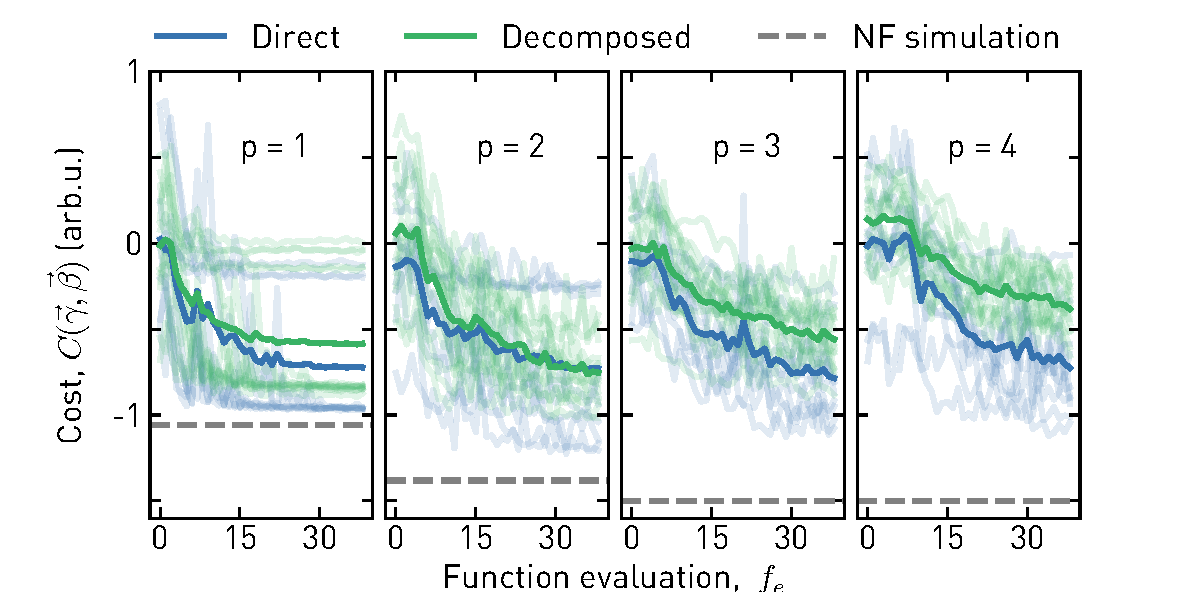
\includegraphics[width=\textwidth]{chapters/qaoa/figs/ch5_qaoa_optimization_traces_one_line_20200205_212444.pdf}
    \caption{Cost optimization trajectories for depths of $p=$ 1, 2, 3 and 4 as a function of the number of function evaluations, $f$. The variational parameters are initialized randomly and then optimized iteratively with the Nelder-Mead algorithm. Each cost value is computed from 20000 single shot measurements. The trajectories obtained with the direct (decomposed) implementation of the \gls{carb} are shown in blue (green). The faded lines correspond to the 15 individual trajectories while the darker color correspond to their average. The grey dashed line indicates the minimal achievable cost for each depth as calculated with a noise-free simulation.}
    \label{fig:qaoa_optimization_traces}
\end{figure}

The motivation for a higher number of layers becomes apparent. For $p=1$, we observe for either implementation three different convergence values of the cost function, two corresponding to the local minima and one to the global minimum, as expected from the three pairs of minima visible in Fig.~\ref{fig:qaoa_landscapes}. The local minima significantly impact the average cost at convergence. In addition, the best case performance is limited by the minimal achievable cost for $p=1$.

For $p=2$, the best trajectories of the direct implementation achieve cost below what is possible with only one layer and local minima are less apparent, although still present. 

 Three layers are required to reach the minimum cost of $-1.5$ in noise-free simulation. But adding layers does not always yield better performance. Indeed, it also results in longer gate sequences, aggravating the effect of decoherence. Moreover, additional layers increase the dimension of the parameter space, resulting in slower convergence, which is clearly visible by comparing the average trajectories for e.g.\ 1 and 4 layers. In fact, the average trajectories suggest 40 cost function evaluations do not allow the algorithm to fully converge for $p > 1$. 

For $p = 1,3,4$, the direct implementation reaches lower cost on average (for $p=2$, only its median is lower), indicating that the gate sequence length plays a major role in the performance of the algorithm. In the next section, we analyze this effect in more details. 

\subsection{Success probability as function of depth}
The previous section suggests there is an inherent trade-off: additional layers increase the performance of the algorithm in theory but also aggravate the effect of sequence-length-dependent errors in experiments. Similar conclusions were found by Alam et al.~\cite{Alam2019AnalysisQubits}. The goal of this section is to analyze how this trade-off affects the two implementations of the \gls{qaoa}.

Note that the (approximate) solution of a problem found with \gls{qaoa} is the measured bit-string after optimization of the variational parameters. Therefore, a crucial metric to assess the performance is the success probability, $P_s$ (see Section~\ref{sec:qaoa_success_prob}) and not the cost function used for classical optimization of the variational parameters. 

To investigate the effect of the depth $p$ on $P_s$ accurately, we seek to mitigate the influence of the classical optimizer on $P_s$ (namely, the influence of local minima and the convergence speed, which are expected to be equal for both implementations). To this extend, we provide an educated initial guess for the variational parameters. Namely, we first find optimal parameters for each depth in a noise-free simulation and provide these theoretically optimal parameters for the initialization of the quantum computer. Under the assumption of equal depolarization, bit-flip and dephasing channels for all qubits, the optimal variational parameters remain nearly the same in a noise-free and noisy environment, according to a recent theoretical investigation~\cite{Xue2019EffectsAlgorithm}. Because coherence times and coherent errors are not exactly equal for all qubits on our device, we additionally optimize locally with up to 20 function evaluations on the quantum computer. 

We show the result of the above-mentioned protocol in Fig.~\ref{fig:qaoa_sequence_lengths}. The success probability for various depths is plotted versus sequence length, $L$, to facilitate the comparison of sequences of similar lengths independently of the implementation. The dashed lines correspond to the expected success probability in a noise-free environment. 

\begin{figure}[ht]
    \centering
    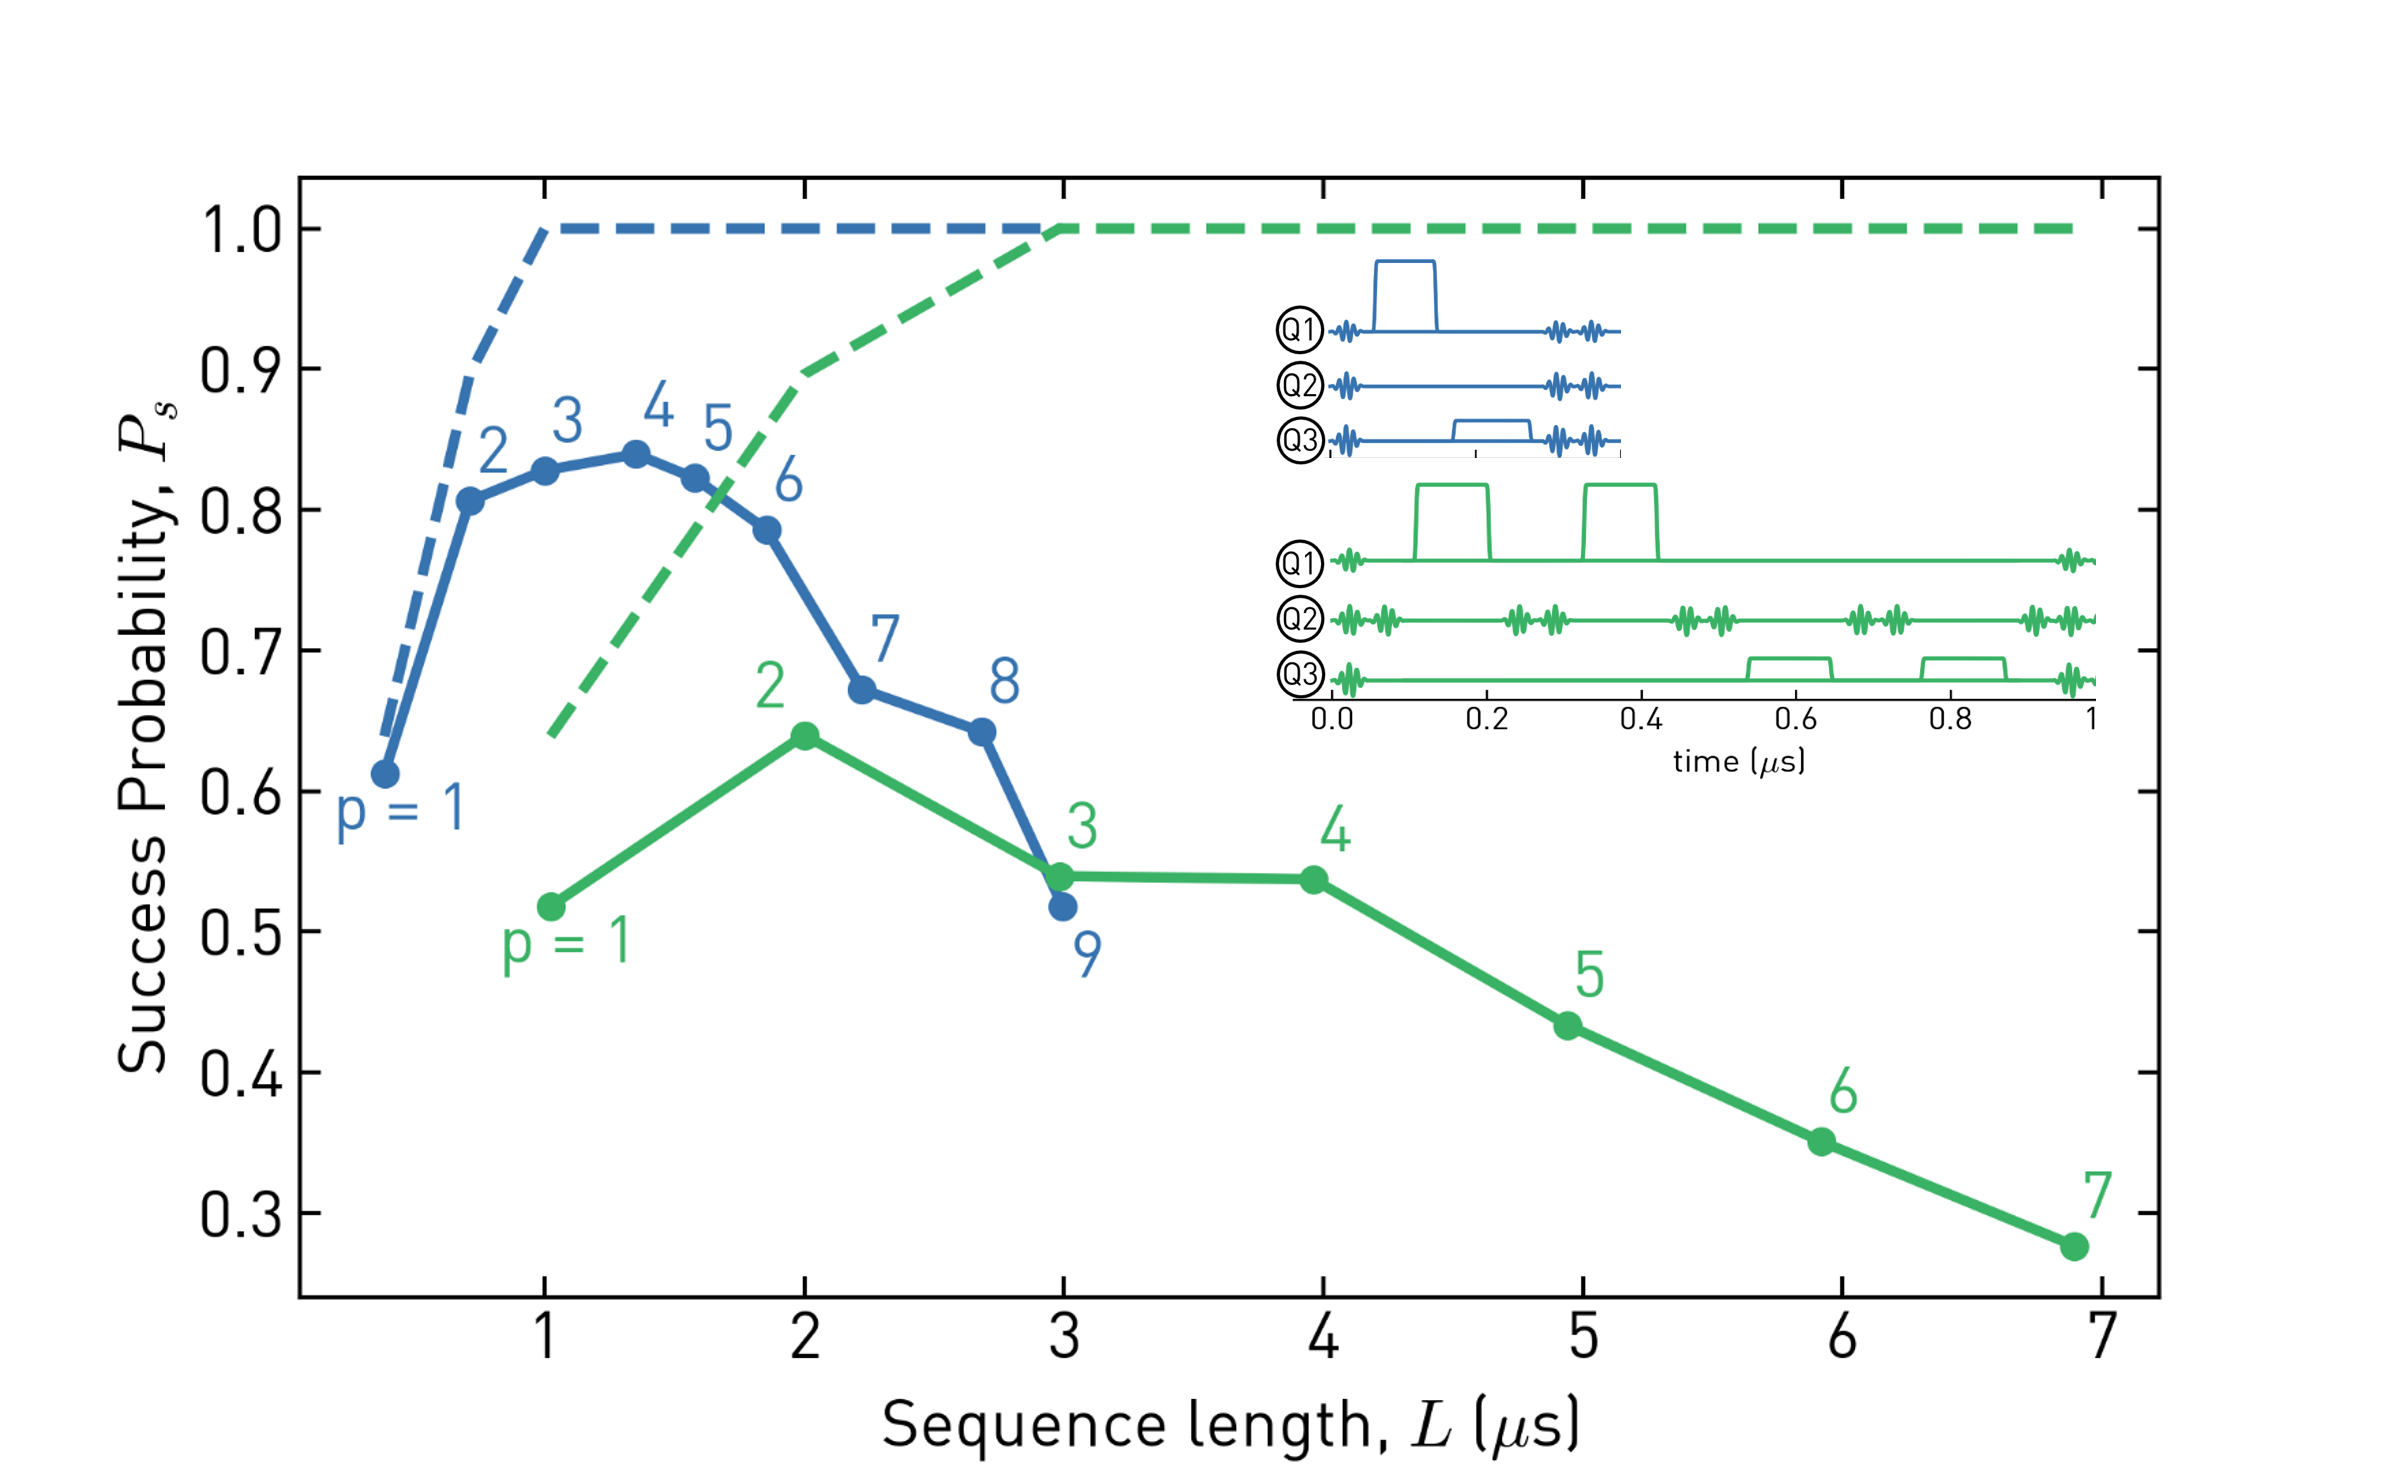
\includegraphics[width=\textwidth]{chapters/qaoa/figs/ch5_qaoa_sequence_lengths_v1_withinset_20200202_120000.png}
    \caption{Success probability as a function of sequence length for the direct (blue) and decomposed (green) implementations of the \gls{carb}. The dashed line of corresponding color indicates the success probability as calculated by a noise-free simulation. The depth is annotated next to the data points. For each depth, the quantum computer is initialized with variational parameters obtained from the noise-free simulation. The corresponding pulse schemes for one layer are shown in the inset.}
    \label{fig:qaoa_sequence_lengths}
\end{figure}

The \gls{dir} exhibits a clear advantage: in about $1\,\mu\text{s}$, it is able to execute a 3 layers of \gls{qaoa} while the decomposed implementation only carries out one. For a fixed depth, it consequently suffers less from errors scaling with the sequence length. 

The difference in sequence length arises from the combination of two factors (see inset of Fig.~\ref{fig:qaoa_sequence_lengths} for the full pulse sequence for $p=1$):
\begin{enumerate}
    \item The decomposition of each \gls{carb} requires two individual \gls{cz} and 4 single-qubit gates. 
    \item The \gls{carb} is shorter than the \gls{cz} for any conditional phase different from $\pi$.
\end{enumerate}
Moreover, the number of \glspl{carb} grows with $\mathcal{O}(m\cdot p)$, where $m$ indicates the number of two-qubit terms in \costh{} which cannot be executed simultaneously. Therefore, the total decomposed sequence length rapidly becomes much longer. 

As mentioned in Section~\ref{sec:qaoa_optimization}, noise-free simulations require in the ideal case 3 layers to reach $P_s \approx 1$, which for the \gls{dec} is realized with $L \approx 3\, \mu\text{s}$. For that sequence length, the \gls{dir} can implement up to nine layers. However, in Fig.~\ref{fig:qaoa_sequence_lengths} we observe that both implementations show similar performance for $L \approx 3\, \mu\text{s}$, which directly indicates that performance is limited by sequence length rather than the number of layers.
In particular, in our case we expect both conditional phase errors due to residual $ZZ$-coupling and decoherence to have a major impact which scales with sequence length.

To gain further insights into the performance of the algorithm, we present in Fig.~\ref{fig:qaoa_state_histogram} the full distribution of measured bit strings for each of the first 4 points ($p=1,2,3,4$ for each implementation) of Fig.~\ref{fig:qaoa_sequence_lengths}. The colored dots in the right panel indicate the respective success probabilities, i.e.\ the sum of the probabilities for states $\ket{010}$ and $\ket{101}$ (colored bars). The right panel also shows the success probability distribution (faded filling) of the optimization trajectories discussed in Section~\ref{sec:qaoa_optimization}. If the trajectories constitute a representative sampling of the parameter space, the dot should lie at the right edge of the distribution. A data point outside the distribution suggests the trajectories did not converge to the lowest possible value, or did not find the global cost optimum, for instance because of a local minimum. Conversely, a data point inside the distribution suggests the initialization from theoretically optimal variational parameters is not perfect, or fluctuating performance compared to when the trajectories were recorded.

\begin{figure}[ht]
    \centering
    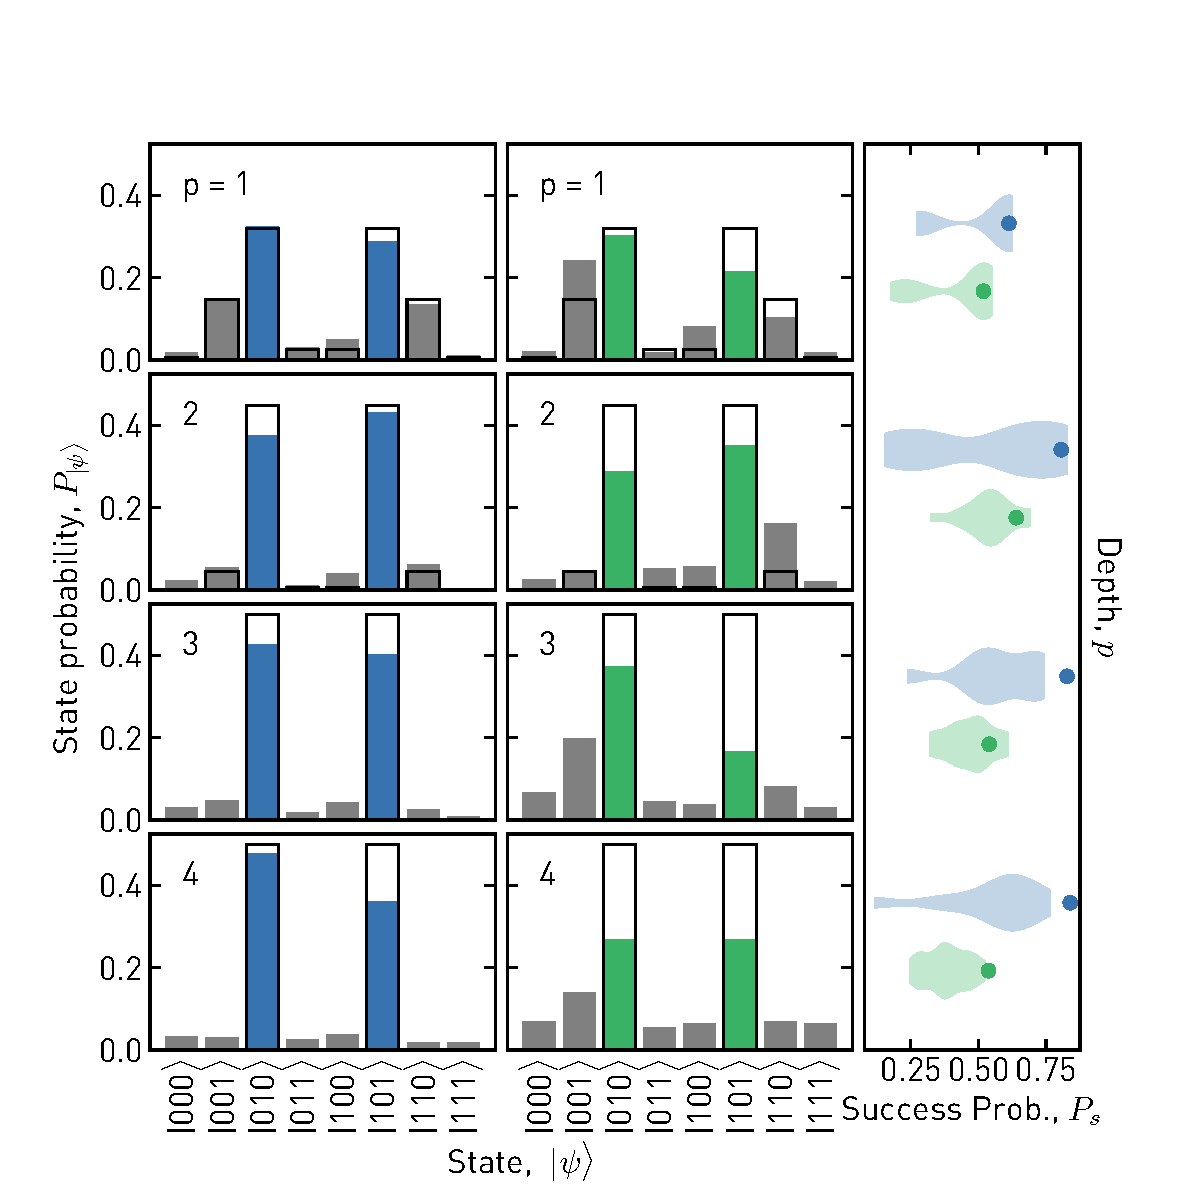
\includegraphics[width=\textwidth]{chapters/qaoa/figs/ch5_qaoa_state_histograms_20200202_134816.pdf}
    \caption{Distribution of measured states for the \gls{dir} (left) and \gls{dec} (middle) for $p=1,2,3,4$. The black wire-frame corresponds to the noise-free simulation distribution of states and is equal for both implementations, at fixed depth. For each distribution, the highlighted bars correspond to solutions of the exact cover problem. Their sum amounts to $P_s$, shown on the right panel with dots of corresponding color (also corresponding to the first 4 dots for each implementation in Fig.~\ref{fig:qaoa_sequence_lengths}). The faded distributions in the right panel correspond to the success probability of the optimization trajectories presented in Fig.~\ref{fig:qaoa_optimization_traces}.}
    \label{fig:qaoa_state_histogram}
\end{figure}

In the state distributions, the most likely states are $\ket{101}$ and $\ket{010}$, corresponding to the desired sets $\mathcal{L}_1' = \{A,C\}$ and $\mathcal{L}_2' = \{B\}$ defined in Section~\ref{sec:qaoa_exact_cover}. The \gls{dir} is in excellent agreement with the noise-free simulation (black wire-frame) for all depths, and achieves a success probability of $0.84$ at $p=4$\footnote{In principle three layers are sufficient to reach $P_s \approx 1$ and additional layers are expected to suffer from additional errors, thereby showing a decrease in success probability. However, the classical optimizer also allows to compensate for some errors and more parameters provide additional degree of freedom to correct for errors.}. By contrast, the \gls{dec} consistently shows more deviations from the simulation and achieves a maximal success probability of $0.64$\footnote{Note that one of the optimization trajectory starting from random initialization reaches a success probability of $0.69$ at $p=2$. We attribute this difference to fluctuations in coherence times and gate performance} at $p=2$. 

We conclude that the trade-off of additional layers affects the two implementations of the \gls{carb} differently. The success probability of the \gls{dir} increases for up to four layers before being decreasing due to decoherence and accumulated phase errors, thereby achieving a success probability of 0.84. On the other hand, the \gls{dec} can only execute two layers before being affected by sequence length dependent errors, which is not sufficient to reach the regime where the success probability is near unity even in the noise-free simulation.

\section{Conclusion}
\glsreset{qaoa}

In this chapter, we have found approximate solutions for a three-qubit exact cover problem instance using the \gls{qaoa}. The problem instance requires at least three layers of the \gls{qaoa} in the ideal case to reach a success probability approaching unity, as determined by noise-free simulations. To the best of our knowledge, this constitutes the deepest problem considered in the experimental \gls{qaoa} literature. 

We have shown that for this problem instance, the direct implementation of two-qubit interaction terms in each layer of the \gls{qaoa} reduces the two-qubit gate-count by 50\% and the executed gate-sequence length by a factor of $\sim 3$ compared to a decomposition into 2 \glspl{cz} and 4 single-qubit gates. Exploiting this advantage, we demonstrate a success probability of $0.84$ using 4 layers of \gls{qaoa}. In comparison, the decomposed implementation reached a maximal success probability of $0.64$ with 2 layers as it is more affected by decoherence and residual $ZZ$-coupling. Experimental observations also strongly suggest that decoherence and residual $ZZ$-coupling are the dominant error sources in both implementations.

The sequence length reduction factor enabled by \glspl{carb} scales approximately linearly with the number of two-qubit terms in the cost Hamiltonian which cannot be executed simultaneously. Typically, the number of two-qubit terms grows with the number of qubits in the problem instance. We therefore expect a considerable performance gain on near-term quantum processors with 10-1000 qubits, as a linear reduction in sequence length avoids exponentially increasing incoherent errors.  In summary, this work provides tangible evidence that \glspl{carb} open the door to solving more complex problem instances on quantum computers for as long as the algorithm's performance are limited by decoherence. 

